\begin{figure*}[t]
\centering
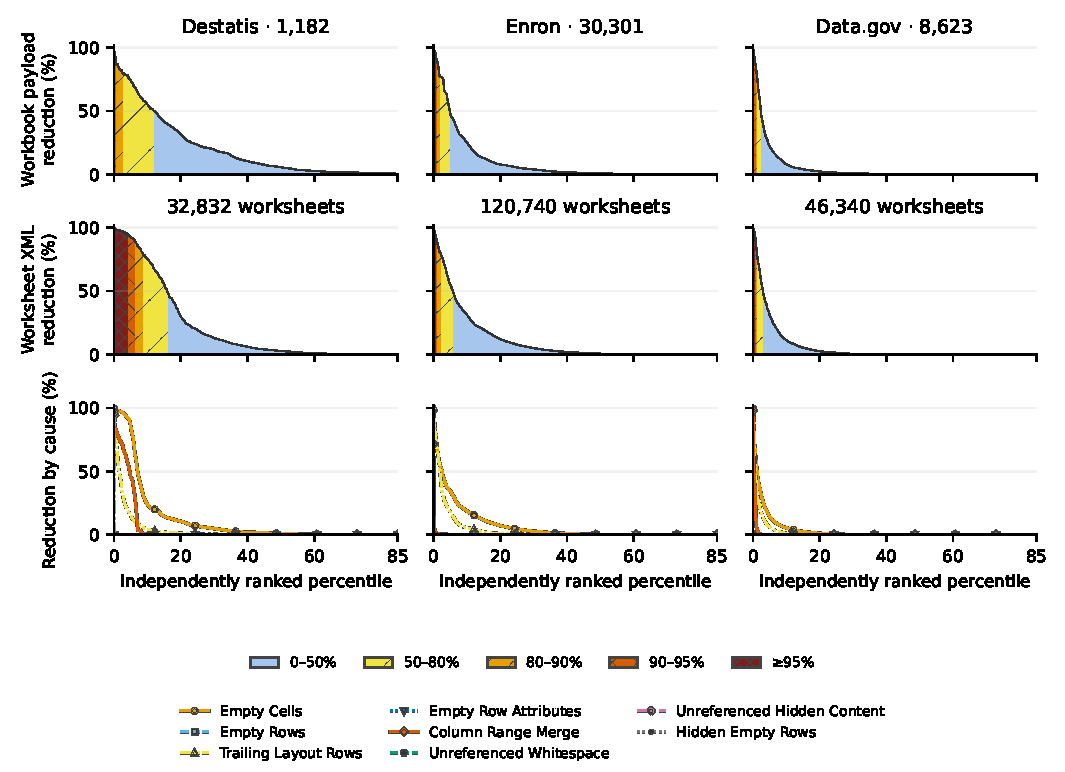
\includegraphics[width=\textwidth]{figures/corpus-uncompressed-distributions.pdf}
\caption{Full-corpus uncompressed-size reduction. Top, complete workbook
payload from all ZIP member sizes recorded in the central directory.
Middle, uncompressed worksheet XML.
Bottom, worksheet XML reduction attributed to each recorded cleanup cause.
Each curve independently sorts its observations from greatest to least
reduction. The x-axis gives the fraction of observations traversed in that
ordering. The common display ends at the 85th percentile. Remaining positive
reductions are below 0.5 percentage points. The omitted tail includes unchanged
outputs and growing workbooks (3/24/5) and worksheets (82/143/39), in
Destatis/Enron/Data.gov order, retained in the accompanying data.
Colors and hatching mark 50/80/90/95\% reduction tiers.
Data.gov's 494 unsupported-namespace
inputs are excluded from these processed-output distributions. The worksheet
panels cover 1,182 Destatis, 30,213 Enron and 8,623 Data.gov workbooks with
recorded worksheet XML. Enron begins with prepared XLSX inputs.}
\label{fig:corpus-distributions}
\end{figure*}
